\documentclass{book}
\author{David Gabriel Corzo Mcmath}
\title{Programación III - Post Parcial}
\date{2019-09-17 07:12}
% % % % % % % % % % % % % % % % % % % % % % % % % % % % % % % % % % % % % % % % % % % % % % % % % % %
\usepackage[margin = 1in]{geometry}
\usepackage{graphicx}
\usepackage{fontenc}
\usepackage[spanish]{babel}
\usepackage{amsmath}
\usepackage{amsthm}
\usepackage[utf8]{inputenc}
\usepackage{enumitem}
\usepackage{mathtools}
\usepackage{import}
\usepackage{xifthen}
\usepackage{pdfpages}
\usepackage{transparent}
\usepackage{color}
\usepackage{listing}
\usepackage{hyperref}
\usepackage{pdfpages}
% % % % % % % % % % % % % % % % % % % % % % % % % % % % % % % % % % % % % % % % % % % % % % % % % %%

\begin{document}
\maketitle
\tableofcontents

\chapter{2019-09-17}
\section{API's \& sus peculiaridades}
\begin{itemize}
\item \textbf{Nos preguntamos:} ¿Por que razón puedo ver el XML en el browser? Es por que estamos usando el método GET.
\item AJAX no permite no tiene la versitabilidad de parser. Este es el defecto de beautiful Soup, para el tipo de interacciónes con AJAX se necesita usar elenioum.
\end{itemize}

\section{Flask}
\begin{itemize}
    \item Flase es un framework, no es como Django que uno es obligado a usar cirtas cosas oblgatoriamente, \emph{\textbf{Definición de ``framework":} es un set de herramientas.}
    \item Usualmente utiliza menos memoria usar ``from <librería> import <funciones o clases a usar>''.
    \item Está corriendo en un puerto.
    \item \emph{\textbf{Definición de ``Socket":} la combinación de una IP  y un puerto}.
    \item Con hostname:
    \begin{verbatim}
        DAVIDCORZO@DESKTOP-73D7DE2 /cygdrive/c/Users/DAVIDCORZO
        $ hostname
            DESKTOP-73D7DE2
    \end{verbatim}
    
    \item app.run(host$=$"0.0.0.0",port=55) el host= 0.0.0.0. permite ver por medio de la red aplicaciones corriendo en otras computadoras.
    \item \emph{\textbf{Definición de ``puerto":} permite cambiar el socket, tiene un máximo de 65,535 puertos}.
    \item Debug igual True, uno de los beneficios que permite es correr la app sin tener que iterar el ciclo guardar,correr,ver\_resultados, pero el chiste es debugging.
    \item En python ``@'' es un decorador, es una manera implicia de llamar funciones.
    \item Cambiémos la ruta con el decorador a ``@app.route("/alumnos)''
    \item En flask hay dos formas de render: \emph{\textbf{Definición de ``Server side rendering":} fui a la base de datos y la respuesta solo al sabe mi aplicación, soy capaz por ende de imprimir información ingresada en mi aplicación.} \emph{\textbf{Definición de ``client side rendering":} este render lo hace el browser.}
    \item Lenguages de renderización, pintar de manera bonita en el browser.
    
    \item In jinja2 se referencia a una variable asi: ``\{\{ <variable> \}\}'', para hacer un for loop \{\% for i in algo \%\}.
\end{itemize}

\section{Averiguar después}
\begin{enumerate}
    \item decorators ``@''
    \item CSS Bootstrap
    \item jinja2 en Flask 
    \item Server side render, client side render.
    \item Leer Redis.
\end{enumerate}


\chapter{2019-09-19}
\section{Subjetivismo}
Es la teoría de valor de acuerdo a lo subjetivo, el comunista piensa que el valor de los bienes son objetivos, un comunista pretende planear todo desde arriba. \newline 
Valor de los bienes es subjetivo, bienes tienen función de acurdo necesidades que satisfacen, tiene valor para alguien y para otra persona pueda que no tenga valor. Si la teoría del valor fuese cierta ninguna empresa quebraría. Si la cantidad de trabajo determina el precio simplemente cualquiera quisiera meterle hasta trabajo de por gusto. \newline 
Teoría de subjetivismo: el valor se determina por qué tan bien satisfacen las necesidades existentes.

\section{Marginalismo}
El marginalismo, la paradoja de el agua y los diamantes, las necesidades o el valor de los bienes viene dado de la necesidad marginal, el ultimo de los fines que permite conseguir, toda decisión se toma al margen. El valor que tiene la unidad, la ultima unidad de algún bien.

\begin{center}
    \begin{figure}[htbp]
        \centering
        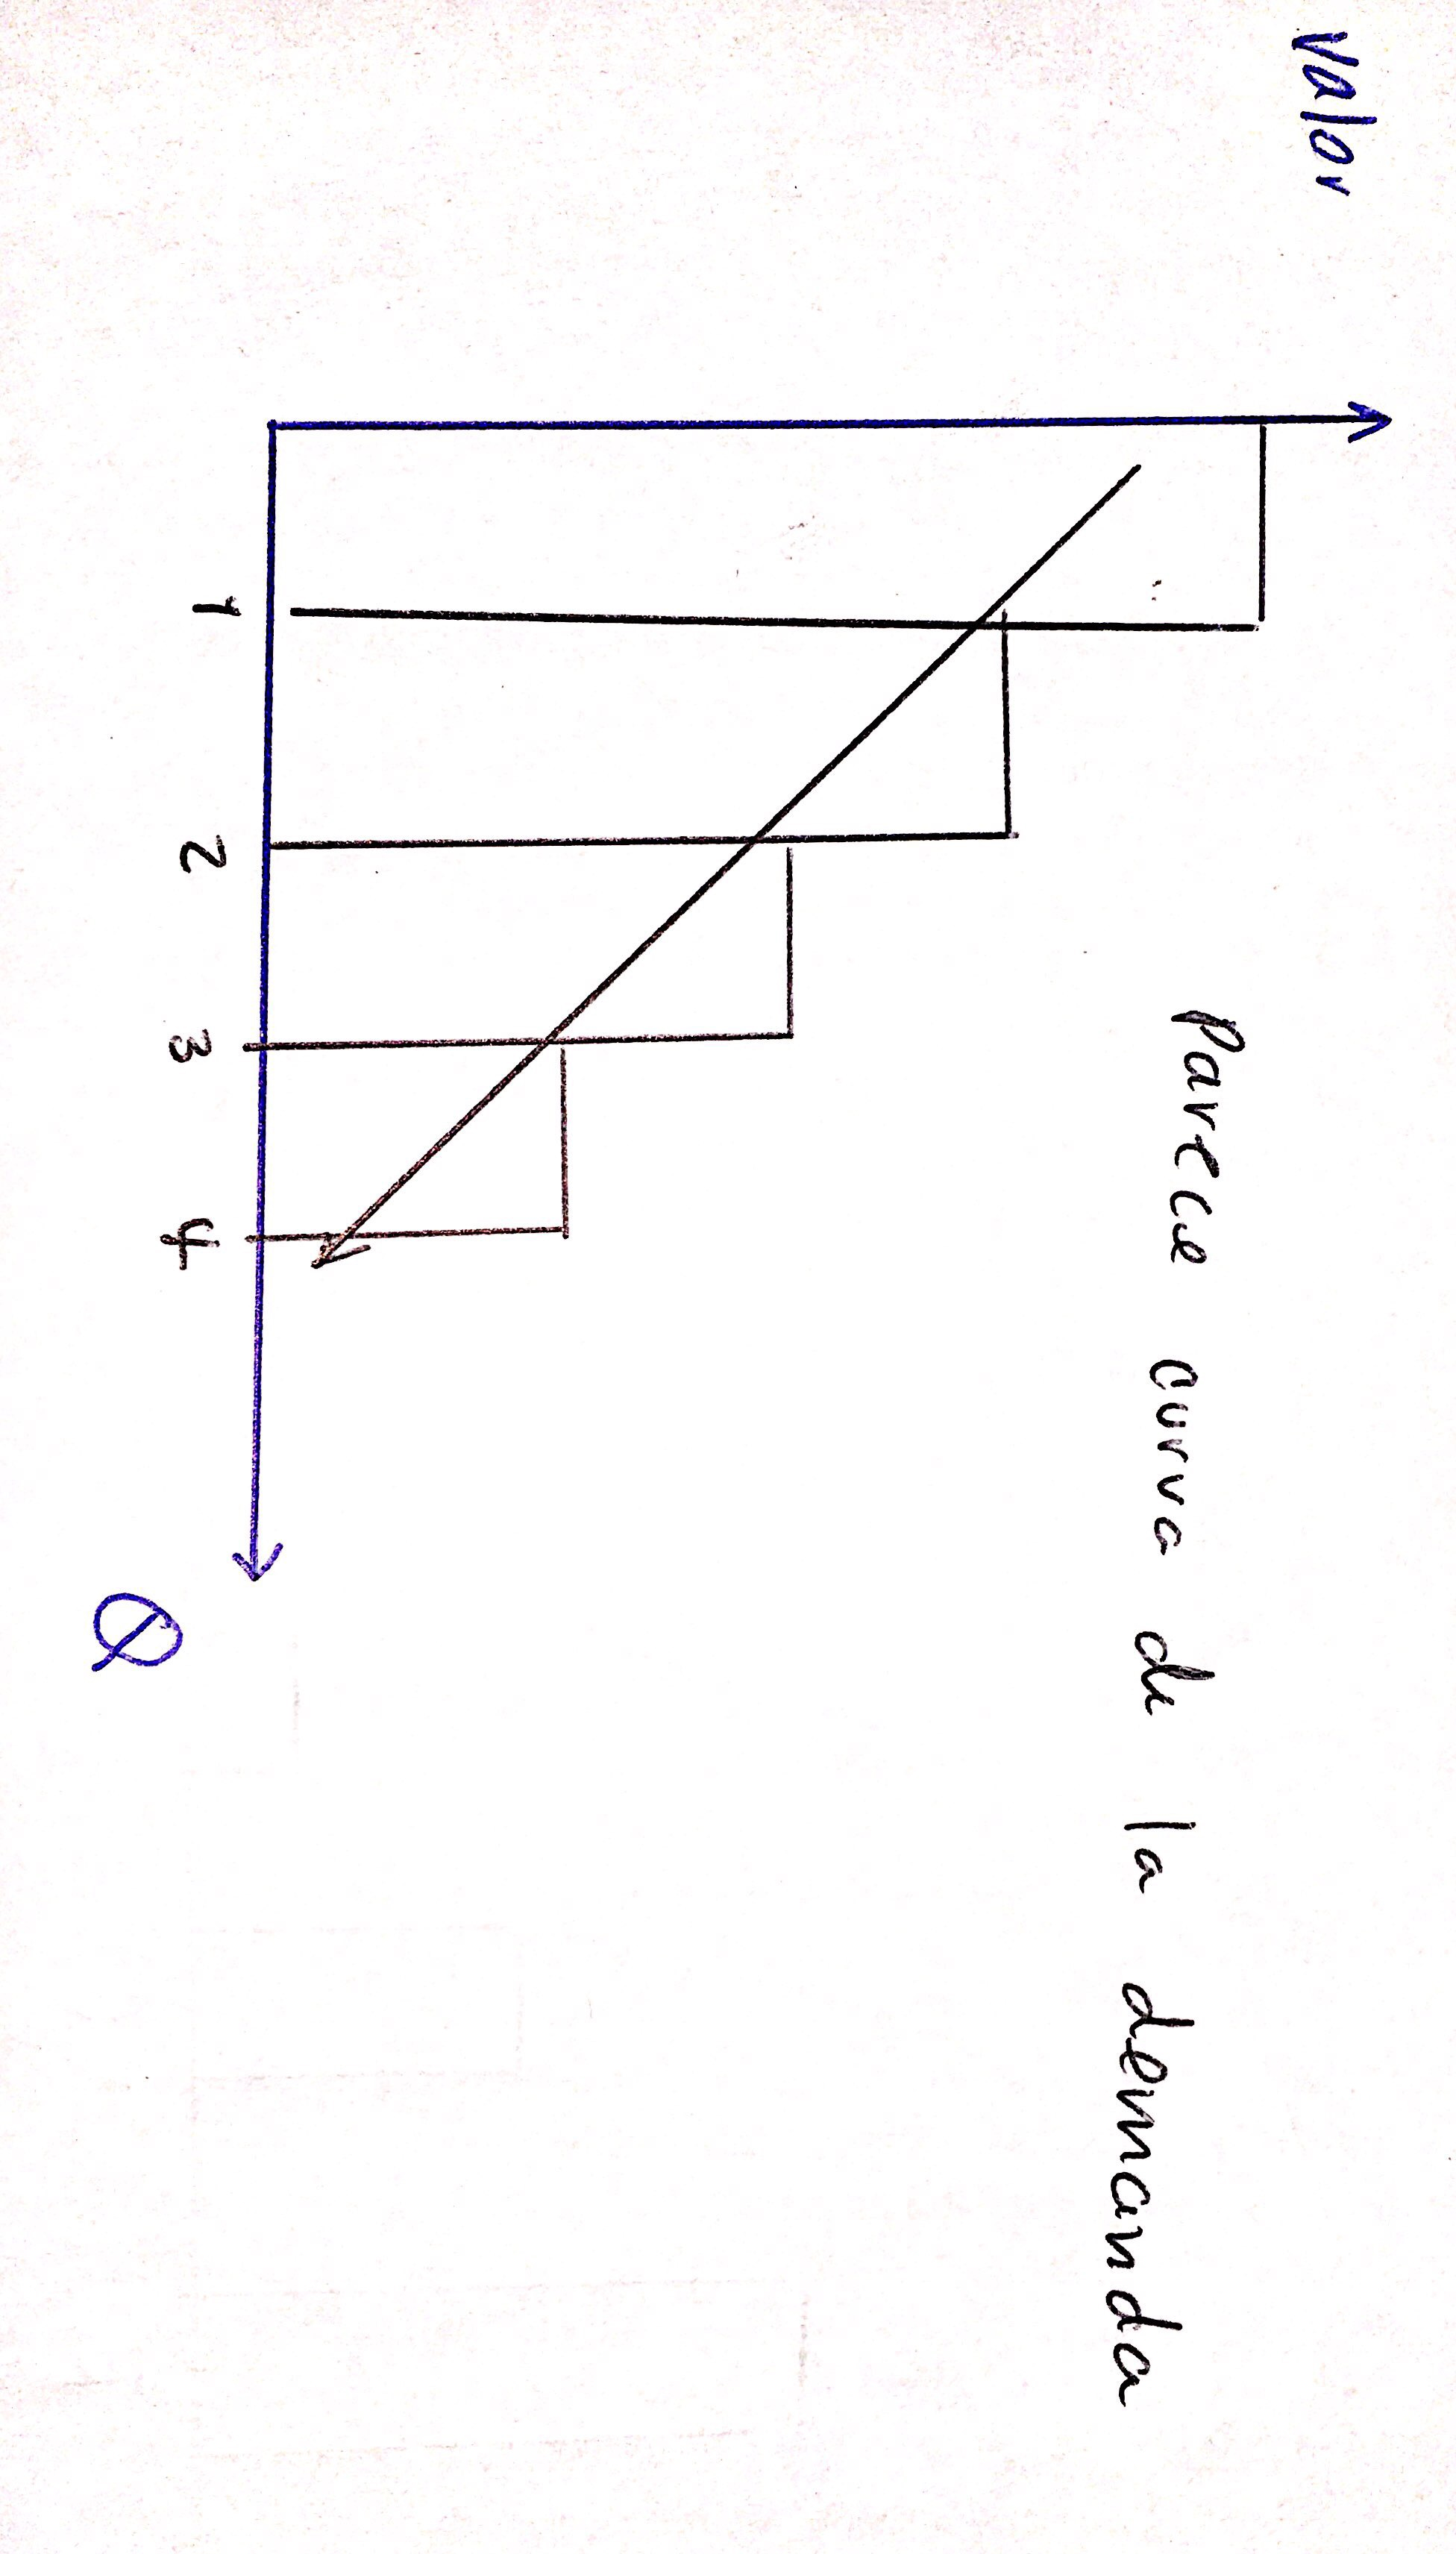
\includegraphics[width=6cm,angle=90]{Classes/Images/2019-07-24-1.jpg}
        \caption{La marginalidad tambien se puede representar como una curva de demanda también}
        \label{fig1}
    \end{figure}
\end{center}

% \vspace{10pt}
\begin{center}
    \begin{figure}[htbp]
        \centering
        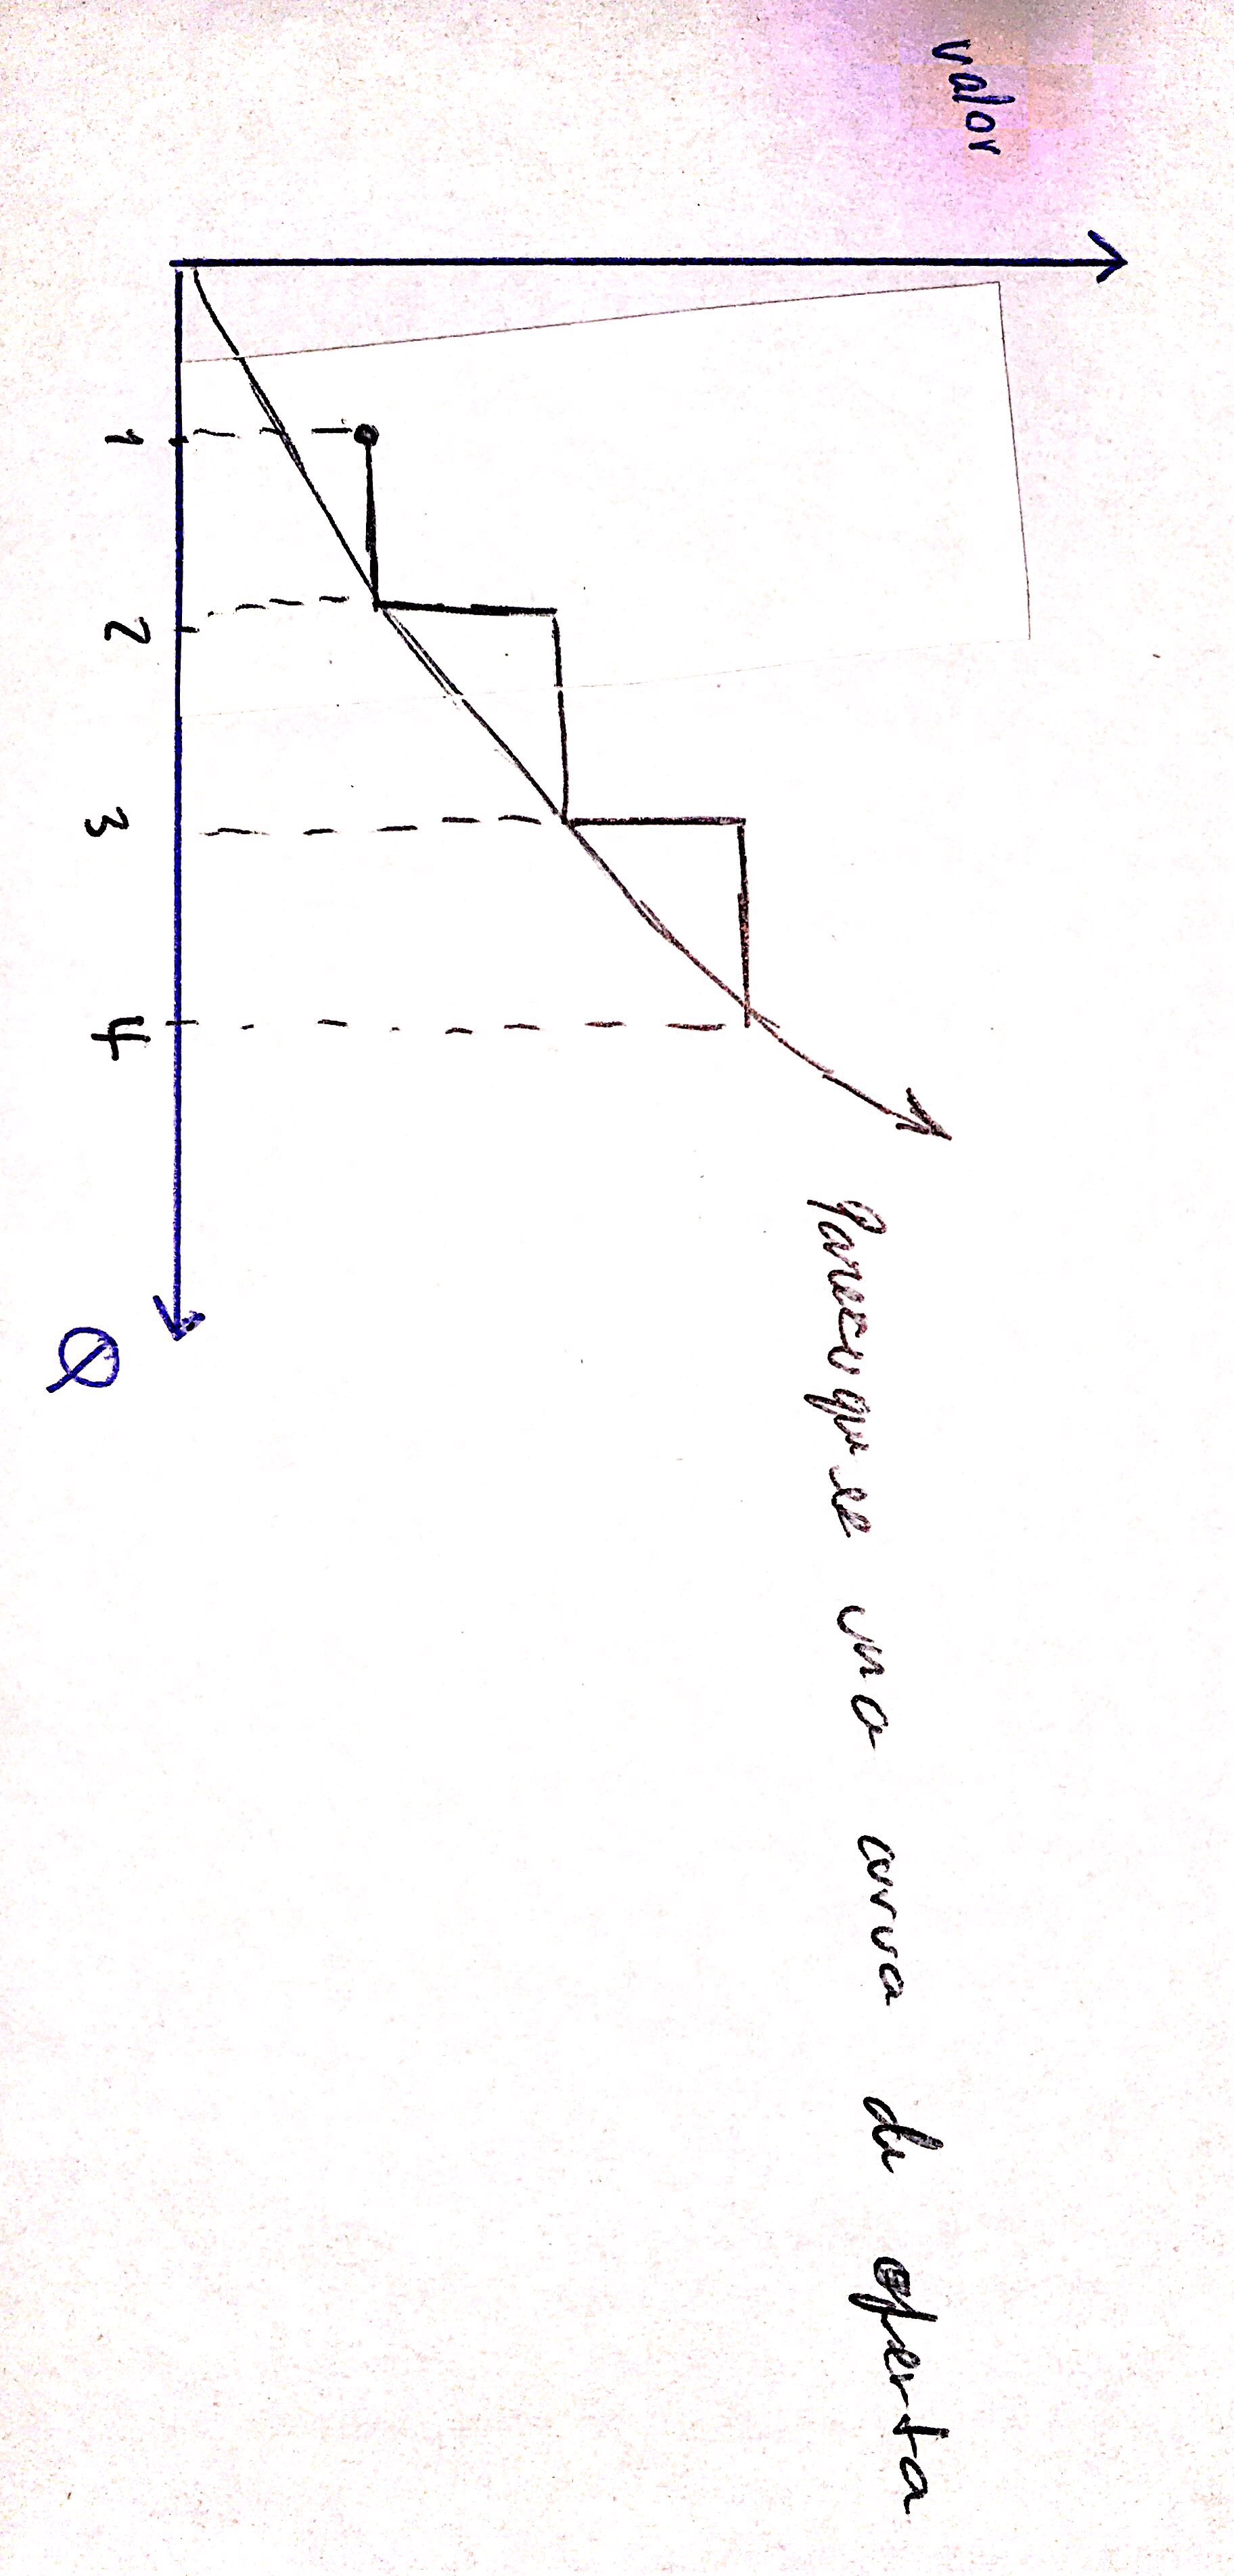
\includegraphics[width=6cm,angle=90]{Classes/Images/2019-07-24-2.jpg}
        \caption{La marginalidad puede interpretarse como una curva de oferta tembién}
        \label{fig2}
    \end{figure}
\end{center}




\section{Oferta y demanda}
Teoría de la utilidad marignal, el principio de utilidad marginal decreciente es \textbf{siempre} decreciente. El reverso de la teoría marginal decreciente coste marginal creciente; la utilida de una unidad más conlleva que todas las unidades van a disminuir de valor.
\begin{center}
    \begin{figure}[htbp]
        \centering
        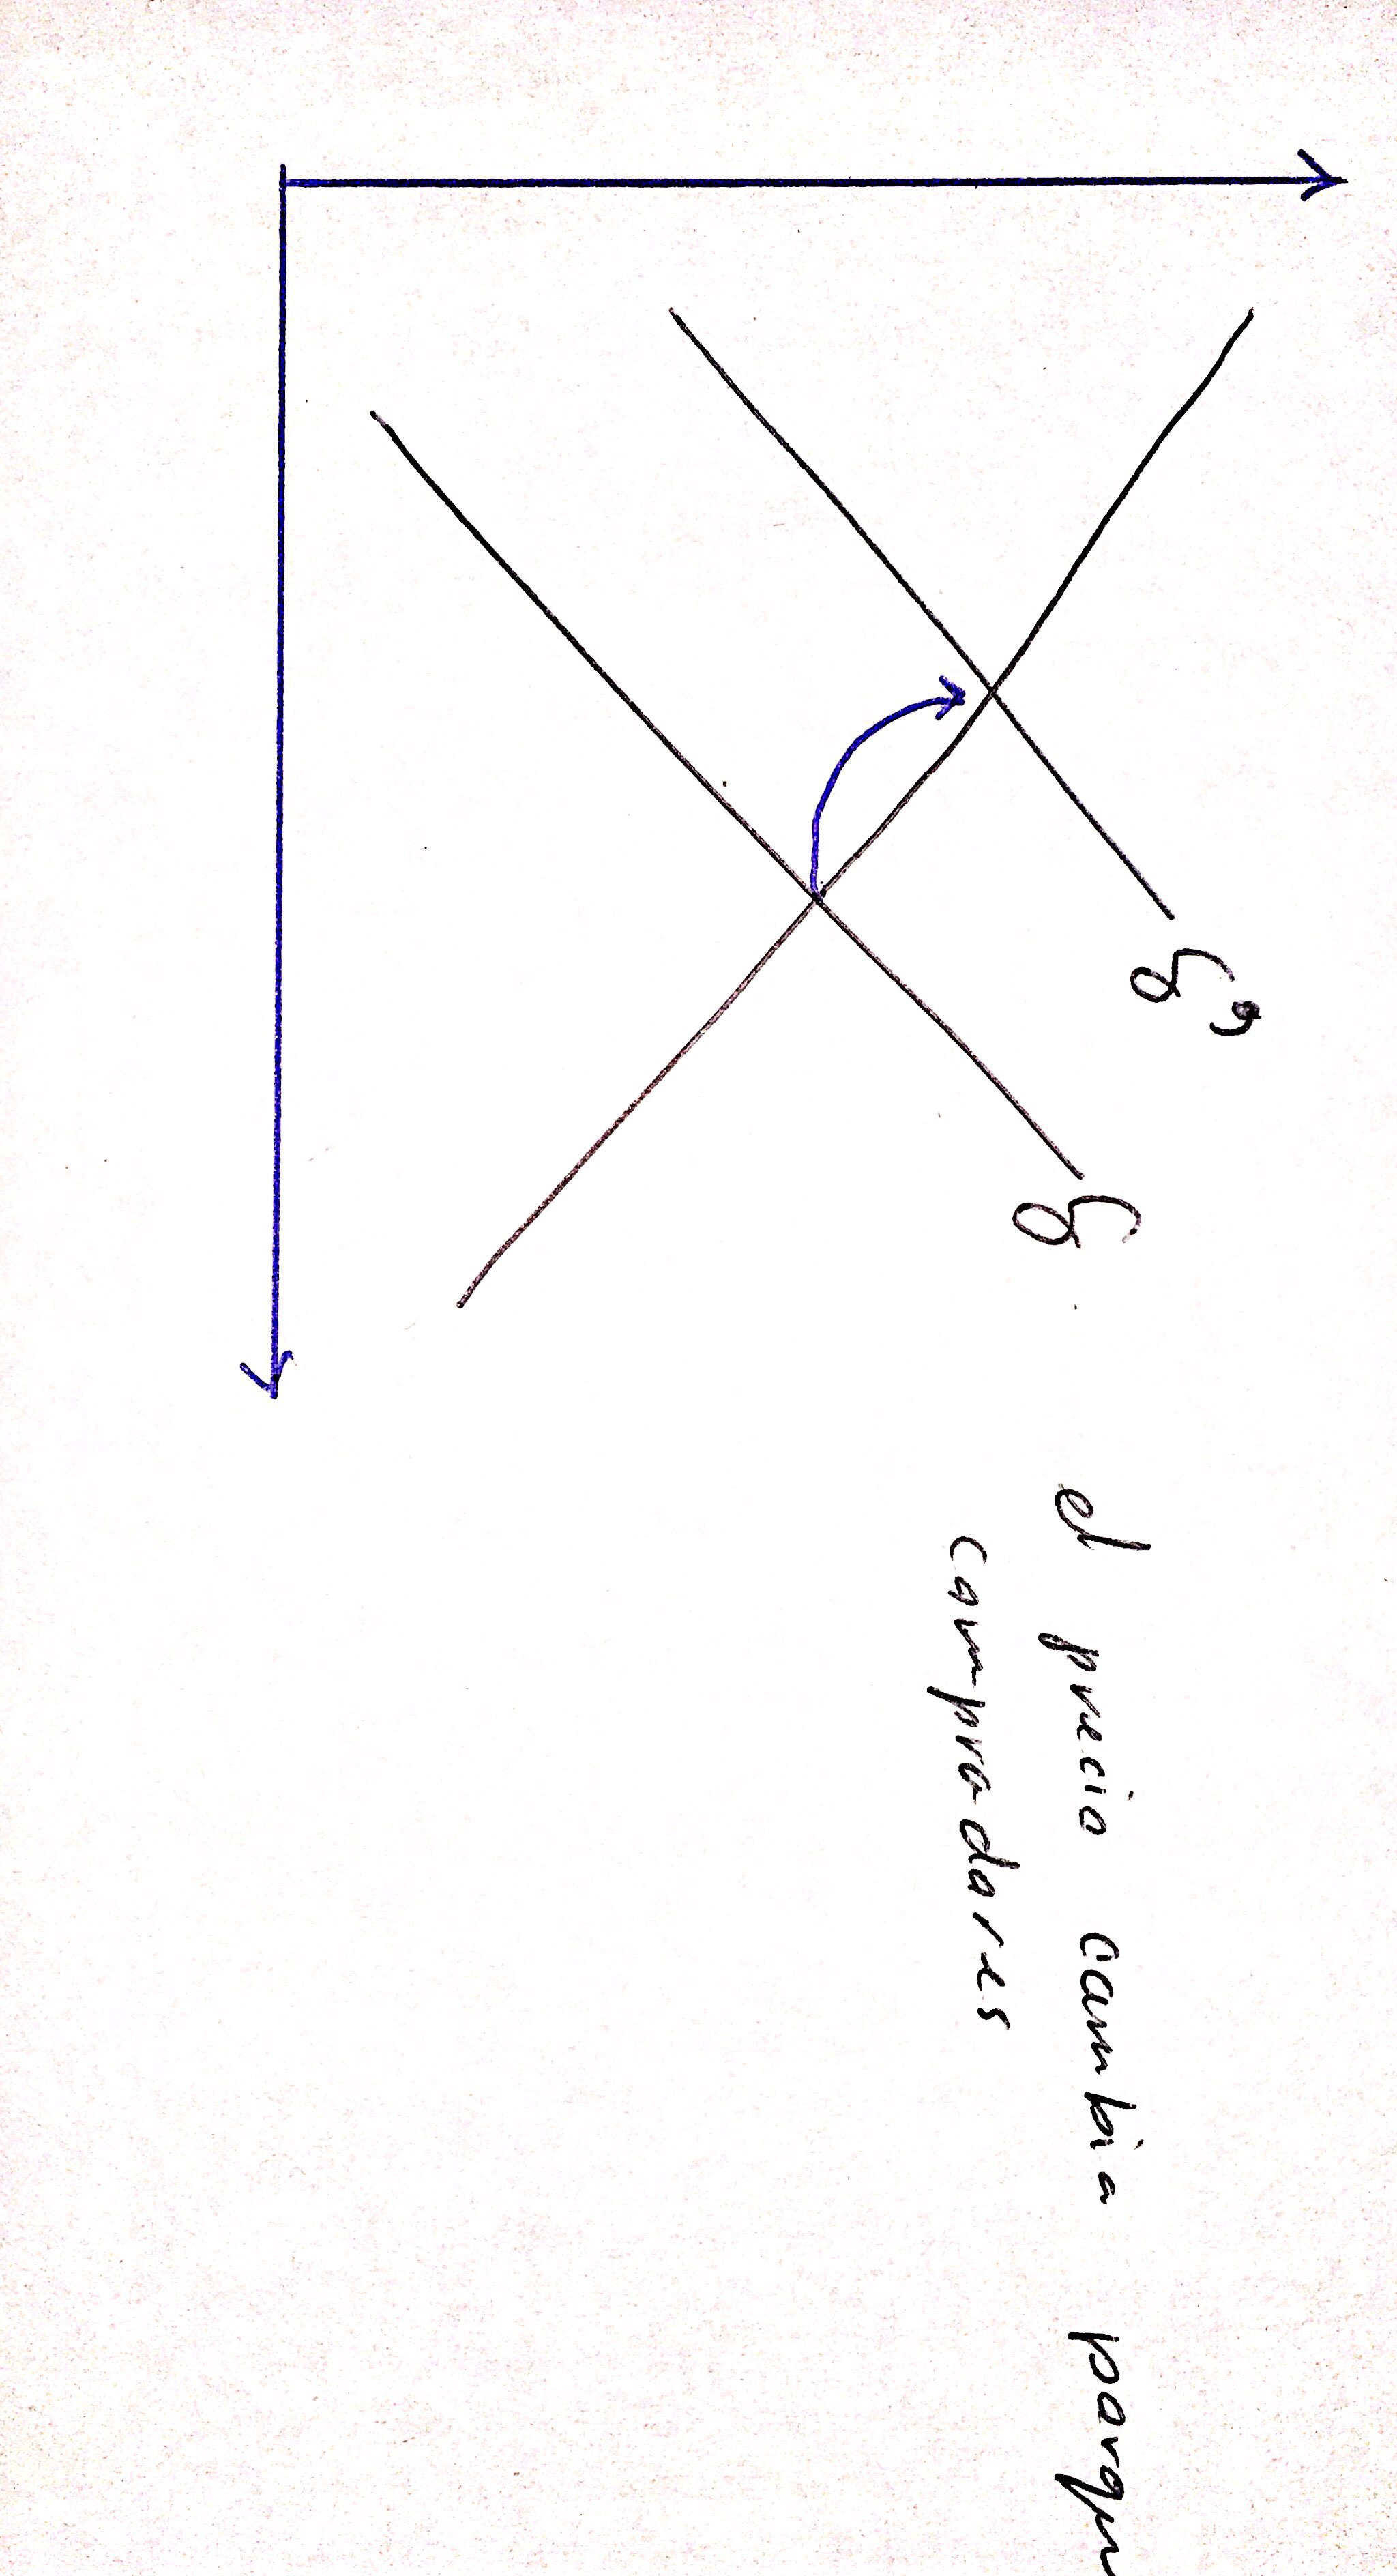
\includegraphics[width=6cm,angle=90]{Classes/Images/2019-07-24-3.jpg}
        \caption{El precio cambia porque los compradores designan una utilidad diferente cada vez y es subjetiva, al igual que los oferentes}
        \label{fig3}
    \end{figure}
\end{center}


\section{Sistema de precios}
Informa de manera indirecta, sobre que producir, con quién producirlo, cuánto producirlo y para quién producirlo. \textbf{Nos preguntamos:} ¿el precio es el determinante o el determinado? El sistema de precio es el determinado. Ejemplo, si un precio sube alguien va a tender a querer meterse a producirlo. El sistema de precios comunica información esencial para que las personas puedan actuar. Es una dinamica de precios que previene la escasez. En general los empresarios persiguen beneficios altos, por eso un empresario le puede parecer mas rentable producir mesas que producir iPhones. Tasa de rentabilidad, qué tanto te vas a tardar en recuperar la inversión. \newline 
Las rentabilidades altas se detruyen con competencia, se tiende a equilibrar, termino 12.27.
% insertar graficas aqui rentabilida.
\begin{center}
\begin{figure}[htbp]
    \centering
    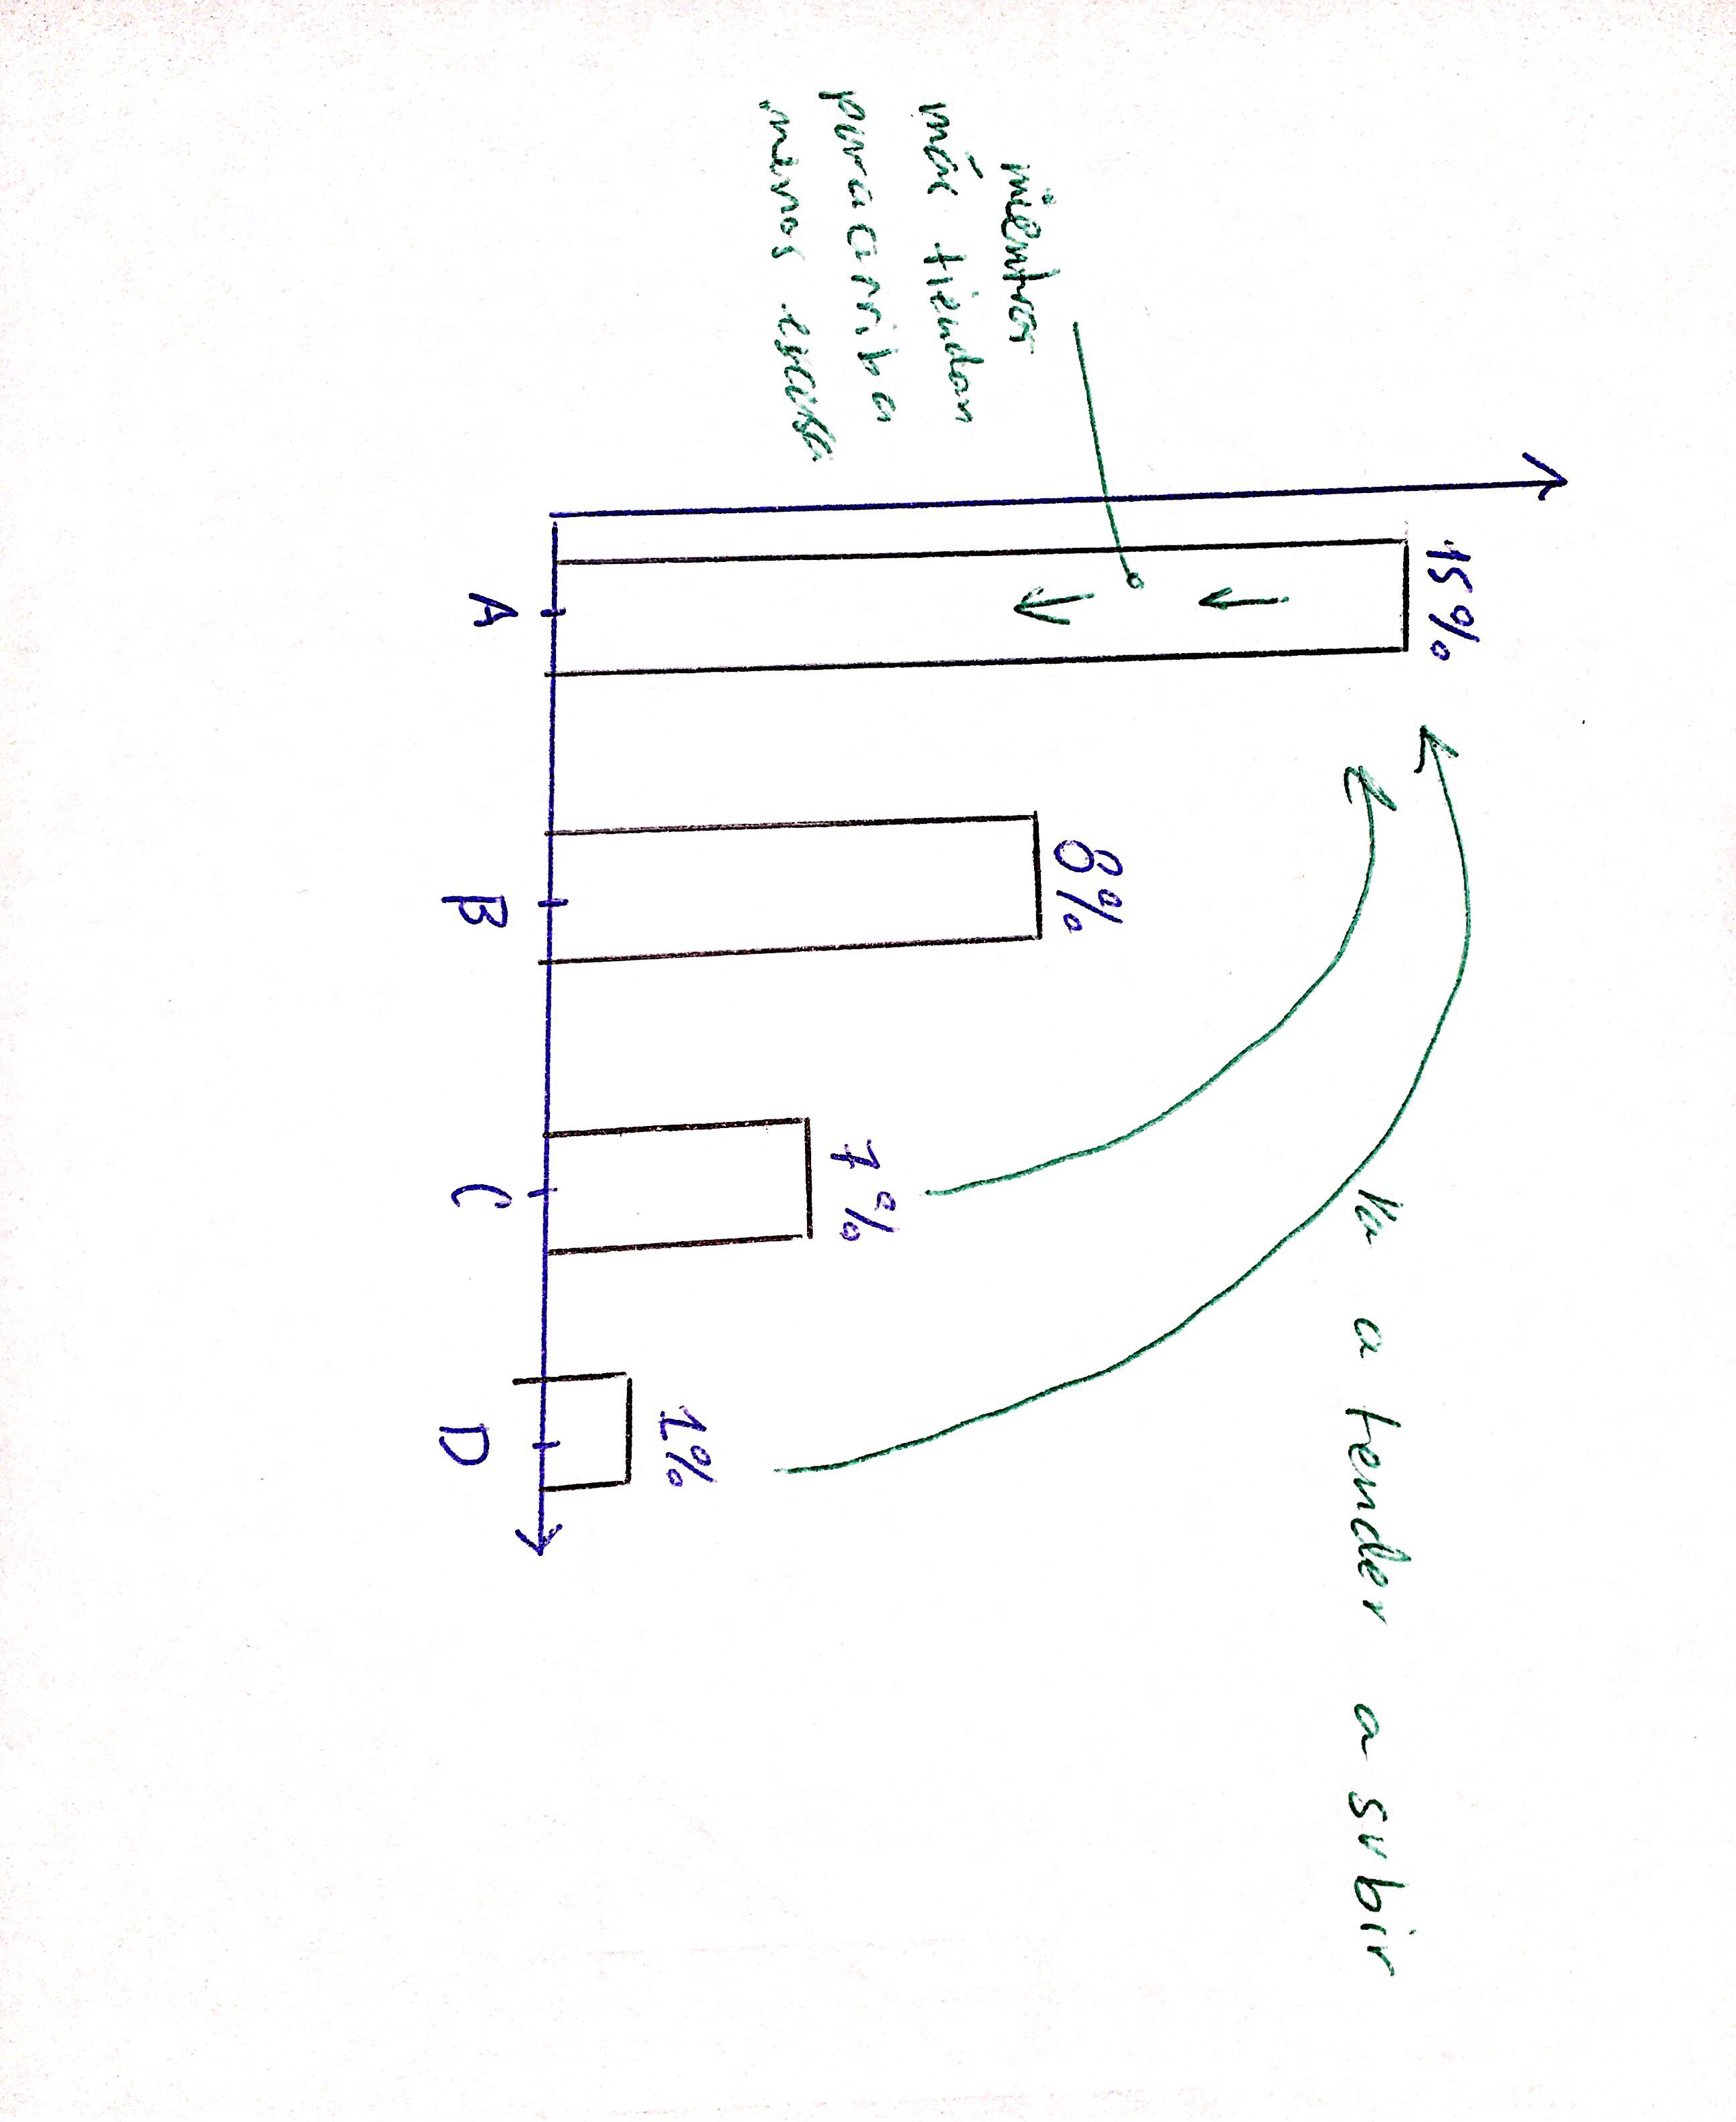
\includegraphics[width=8cm,angle=90]{Classes/Images/2019-07-24-4.jpg}
    \caption{Tiende al equilibrio}
    \label{fig4}
\end{figure}
\end{center}


\section{Subcidios e impuestos}
Si quieres más de algo lo subsidias, si quieres menos de algo pones impuestos. \textbf{Ejemplo: } los ecofiltros regalados, los usaban para masetas, se sobre utiliza. \newline 
\textbf{Ejemplo: } Impuesto a gasolina, se hace caro y la gente lo consume menos. 

\section{Fijación de precios}
Cuando ponen un precio tope se producen faltantes, \textbf{Ejemplo: } el precio de arroz es 3, se presume que es para que toda la gente lo pueda comprar, pero se produce información distorsionada en el sistema de precios y la gente lo empieza a ya no valorarlo. \textbf{Ejemplo: } Venezuela, se controla el harina y el pan, lo que termina produciendo es que todas las panaderías están vacías, si se ponen precios topes se agotan en seguida y nadie le sale rentable producir entonces no se produce. \textbf{Ejemplo: } Los taxis, están a punto de ser erradicado, hay precio minimo de 25Q y ahora lo que ocurre es que los taxis ya no se usan, el precio tope busca controlar la oferta. \textbf{Ejemplo: } El salario mínimo, mientras más pujan el precio del salario minimo para arriba, se aumenta la demanda y se disminuye la oferta, todas las cosas como seguro social, aguinaldo, bono 14, y el salario mínimo termina siendo carísimo. 

\section{Noticia}
Quiz el lunes de la lectura, resumir y analizar la noticia en 5 minutos. 



\chapter{2019-09-24}
\section{Espacio marítimo y espacio aéreo}
El estado comprende los espacios marítimos siguientes:
\begin{enumerate}
    \item Mar territorial: En Guatemala son 12 millas náuticas, \emph{\textbf{(Paréntesis:}La milla terrestre no es igual a la milla nautica aprx. 0.8km = 1 milla náutica)}
    \item Aguas interiores
    \item Zona económica exclusiva: 200 millas náuticas desde la costa
    \item Zona contigua: 24 desde la costa
    \item Plataforma continental \newline 
    --------------------------------------------
    \item Alta Mar: No forma parte del territorio de un estado. Comprende las partes del mar no incluidas en la zona económica exclusiva. Hay plena libertad de todo.
    \item La zona: No forma parte del territorio de un estado. 
\end{enumerate}

\section{Espacio marítimo}
\textbf{Convención sobre el derecho del mar}: es una convención sobre el derecho del mar, se establece todo como qué medidas cuánto, las medidas del mar territorial. \newline 

\subsection{Derechos el estado Ribeño}
\begin{center}
\begin{tabular}{ | c | c | }
\hline
 Todos los que implique el ejercicio de su soberanía & Por ejemplo: Regular navegación, pesca, investigación  \\
\hline
 Derechos de otros estados & NINGUNO \\  
 \hline
\end{tabular}
\end{center}

\subsection{Zona contigua}
\begin{itemize}
    \item Zona de mar adyacente al mar territorial hasta una distancia de 24 millas marinas contadas desde la líneas de base a partir de las cuales de mide el mar territorial.
    \item \textbf{Derechos del estado}: tomar medidas de fiscalización para prevenir las infracciones aduaneras, fiscales, de inmigración, o cuestiones sanitarias:
    \item \textbf{\emph{Ejemplo:}} Si un barco no identificado se va acercando a la costa y es un potencial peligro al estado no es considerado un paso inocente y se necesita solicitar permiso al estado.
\end{itemize}

\subsection{Derechos de los otros estados}
Derechos de paso inocente:
\begin{itemize}
    \item Se permite pasar simplemente, el barco del aborto por ejemplo no era un paso inocente.
    \item Los cruceros estarían cruzando en la zona contigua, si quiere entrar al mar territorial se necesita pedir permiso al estado.
    \item \textbf{\emph{Definición} :Son pasos que alteran la seguridad de alguna manera en el estado.}
\end{itemize}

\subsection{Zona Económica exclusiva}
\begin{itemize}
    \item 
\end{itemize}

\subsection{Derechos del estado ribereño}
\begin{itemize}
    \item Tiene derechos de soberanía para fines de exploración y explotación, conservación y administración de los recursos naturales vivos y no vivos del lecho y el subsuelo del mar.
    \item Se puede hacer islas en la zona económica exclusiva.
\end{itemize}

\subsection{Borde exteriores de la plataforma continental}
\textbf{\emph{Definición} :Es el lecho de el subsuelo que se encuentra de bajo del suelo del mar, se pueden tener cables, se pueden hacer perforaciones siempre con el consentimiento del estado, fondos marínos y oceanos y su subsuelo fuera de los límites de la jurisdicción nacional.}\newline 
\textbf{\emph{Ejemplo:}} Brooklin 99


\section{Espacio aéreo}
\textbf{\emph{Definición} : el espacio que existe entre la atmósfera y el territorio de un estado} \newline 
Es esencial por:
\begin{itemize}
    \item Mantenimiento de seguridad y defensa del estado
    \item Transporte aéreo
\end{itemize}

\subsection{Tipos de espacio aéreo}
\begin{itemize}
    \item Controlado: aquel espacio donde una torre de control por herramientas como radar se establece un espacio aéreo Controlado
    \item No controlado: \textbf{\emph{Ejemplo:}} torre de control de la aurora y torre de control en peten, pero cuando se fumiga con aviones en fincas solo se avisa cuando se usa el avion para comunicar que uno va a estar en el aire.
    \item Espacio aéreo de uso especial: Con propósitos mas que todo militares, es como un territorio que usa el militar para prácticas de soldados por ejemplo.
    \item Derechos sobre el espacio aéreo: qué se puede hacer.
    \item En cuanto a una línea recta no hay, simplemente se establecieron ciertos criterios.
    \item Libertades del aire: 8 libertades principales, los derechos que tiene un estado.
    \item Se clasifican en libertades técnicas y libertades comerciales.
\end{itemize}

\subsection{Derechos de espacio aereo}
\begin{enumerate}
    \item Libertad de pasar sin aterrizar.
    \item Falla técnica, tiene derecho a aterrizar por emergencias. \textbf{\emph{(Ejemplo:una señora se sentía mal en un vuelo de EEUU a Guatemala, se tuvo que seguir un protocolo que atrasó 1:30h y media.)}} Referente a vuelos internos.
    \item Libertades comerciales: desembarque \textbf{\emph{(Ejemplo: pasajeros, correo y carga tomados en el territorio del país cuya nacionalidad posee la aeronave.)}} Involucra lucro. Referente a vuelos internos.
    \item Embarcar, es una libertad comercial de embarque. Involucra lucro.
    \item Poder embarcar y desembarcar en cuanto matrículas de estados diferentes.
\end{enumerate}

\subsection{Espacios ultra-terrestres}
\begin{itemize}
    \item Son espacios como la luna y otros cuerpos celestes
    \item Regula en cuanto a lo que el ser humano pueda mandar a la orbita, ya que despues de cierto tiempo se convierte en desechos
    \item Los cuerpos celestes son patrimonio común.
    \item Regulación constitucional:
    \begin{itemize}
        \item Art. 121 literal b
        \item Art 142 literal a 
    \end{itemize} 
    \item Dirección general de aeronáutica civil
    \begin{itemize}
        \item Regulada en el decreto número 93-2000
        \item Art 3
        \item Art 7 literal a
        \item Art 66
    \end{itemize}
    \item Los derechos de la política de cielos abiertos: reconocer el embarque y desembarque de naves de diferente nacionalidad.
\end{itemize}

\subsection{En Guatemala}
\begin{itemize}
    \item Regulación de drones:
    \begin{itemize}
        \item Aeronaves no tripuladas
        \item Necesidad de registro
    \end{itemize}
    \item Globos aerostáticas:
    \begin{itemize}
        \item RAC 31
    \end{itemize}
    \item Vuelos en parapente y ala delta:
    \begin{itemize}
        \item RAC 103
    \end{itemize}
\end{itemize}

\subsection{Tarea}
\textbf{}   


\chapter{2019-10-01}
\section{Elementos posteriores del estado}

\subsection{El poder}
\begin{itemize}
    \item El poder: En la antigüedad, se necesitaba el estado, la gente buscaba el poder en gobernantes que consideraban dignos de gobernar. 
    \begin{itemize}
        \item El estado \textbf{\emph{Caso ``Juan Sitierra": Era un gobernante }}, se buscaba orden. no puede existir sin poder, no puede existir sin llegar a su fin tempora. y no se puede llegar al fin sin poder. El estado impone el orden a través del poder.
        \item Orden:Se considera mucho el orden, tiene que haber orden.
        \item Poder (autoridad): poder no es absoluto
    \end{itemize}


    \item Características del poder:
    \begin{enumerate}
        \item No es absoluto, \textbf{\emph{Definición: Absoluto es un poder sin límites, como Luis XIV}}, lo que más regula el comportamiento de los gobernantes es la \textbf{Constitución}, hoy en día se tiene límites.
        
        \item Supremo o soberano; es supremo pero no absoluto, el poder es el máximo poder de un territorio y todo lo que conlleva su territorio, es supremo y soberano, el poder esta por encima de todos los demás poderes.
        
        \item Poder de derecho = ordenamiento jurídico; \textbf{\emph{Caso ``Quiché": El mismo pueblo indígena en Nebaj se da el caso de derecho indígena. Es más una ausencia de la autoridad.}}, significa que está determinado por un ordenamiento jurídico.
        
        \item Poder de dominación = Coacción; \textbf{\emph{Definición:  El estado puede ejercer su poder por coacción, o por fuerza.}}
    \end{enumerate}

    
    \item Tareas del poder
    \begin{center}
    \begin{tabular}{ | p{6cm} | p{8cm} | } 
     \hline
    Gobernar & Administrar \\
    \hline
    Dirección de los ciudadanos & Organización de la función administrativa \\
    \hline
    Se gobierna a persona & Se administran cosas \\ 
    \hline
    Mandatos & Satisfacción de necesidades COLECTIVAS \textbf{\emph{(Ejemplo: Carreteras, servicios, públicos)}} \\
     \hline
    \end{tabular}
    \end{center}

    Administrar \textbf{\emph{Definición: se refiere mas que todo a prestar servicios públicos}} \newline 
    Gobierno \textbf{\emph{Definición: Formular mandatos para la conservación dek estado y para el logro de sus fines.}}

    
    \item Soberanía:
    \begin{itemize}
        \item \textbf{Nos preguntamos:} ¿Cómo definirían la soberanía? \emph{(\textbf{Respuesta}:Es el poder supremo. y soberano es })
        \item Art. 141 Constitución; La subordinación entre las ramas del estado es prohibida \textbf{\emph{Caso ``Baldeti y la corrupción": Daba dinero a diputados para aprobar ciertas leyes.}}
        \item \emph{\textbf{(Paréntesis:}Las ramas del estado, ejecutivo, legislativo y judicial. El Art. 141 frena a los tres poderes entre sí)}
        \item El sujeto de la soberanía es el estado: 
        \begin{itemize}
            \item Doctrinas de la soberanía Absolutista, popular y soberanía nacional.
        \end{itemize}
    \end{itemize}

    
    \item ¿Cómo se debe ejercer el poder público en Guatemala?
    \begin{itemize}
        \item Art. 152 Poder público: El poder que ejercen las autoridades públicos del estado. Como se transmite la soberanía a alguien para poder ejercer el obierno y administración.
        \item Art. 153 Imperio de la ley: la ley se extiende a todos sean extranjeros o nacionales se aplica la ley Guatemalteca.
        \item Art. 154  Función pública: \textbf{\emph{(Ejemplo: Los juramentos de jurar defender la constitución)}}
        \item Art. 155 Responsabilidad por infracción a la ley: \textbf{\emph{(Ejemplo: si un funcionario comete un delito, por el hecho de ser funcionario se duplica la pena por el delito.)}}
        \item Art. 156 No obligatoriedad de órdenes ilegales: Ningún funcionario es obligado a obedecer algo que no es legal.
    \end{itemize}

    
    \item El fin es el Bien común: 
    \begin{itemize}
        \item Fin de un estado definido en la Constitución: Art. 1 de la constitución. 
        \item Art.1 Constitución de Guatemala
        \item ¿Cómo definirían el Bien Común? \textbf{\emph{Definición: Bien común, es el conjunto de condiciones sociales, económicas, culturales, morales y espirituales para desarrollarnos}}
        \item \emph{\textbf{(Paréntesis:}En el preámbulo de la constitución de Guatemala, se establece que se va a preferir por default el bien común sobre el bien individual.)}
    \end{itemize}

    \item \emph{\textbf{(Paréntesis:}Razón del estado, teoría que sostiene que el individuo está a la disposición del estado. La teoría de derecho natural, Guatemala sostiene esta teoría ya que el estado esta al servicio de el individuo, es al revéz que la razón del estado.)} \emph{\textbf{(Paréntesis:}Libertad de credo la asegura la constitución pero así como no hay idioma oficial la constitución está escrita en español, asi mismo pasa con la religión Art. 36 Libertad de religión)}
    
    \item Orden jurídico
    \begin{itemize}
        \item \textbf{Nos preguntamos:} ¿Qué entienden por orden jurídico? Ultimo elemento posterior es el orden jurídico, el estado esta sujeto a normas internas y externas.
        \item Estado con otros Estados = Normas de Derechos Internacionales
        \item Estado con Gobernados = Normas Jurídicas Internas
    \end{itemize}

    
    \item La necesidad del derecho en un estado.
    \begin{itemize}
        \item No se concibe al Estado sin Derecho ni al  Derecho sin Estado. 
        \item “Un Estado sin poder soberano es inconcebible, y un Estado con poder que no esté limitado por el Derecho, no es Estado sino fenómeno de fuerza”
    \end{itemize} 

    \item \emph{\textbf{(Paréntesis:}El derecho y el estado según mucho sautores son lo mismo pero en este curso se tratarán como diferentes por la razón que es un ordenamiento jurídico.)}
\end{itemize}

\subsection{Noticia: Conflicto Mexico-Guatemala}
\begin{itemize}
    \item Conflictos acerca de tala de arboles en Petén.
    \item El bombardeo de los barcos.
    \item México corta lazos diplomáticos.
    \item Se resuelve el conflicto.
    \item \emph{\textbf{(Paréntesis:}Relacionar con la soberanía Guatemalteca.)}
\end{itemize}

\begin{itemize}
    \item Sealand
\end{itemize}




\chapter{2019-10-08-Clase de UX}
\section{Diferencias entre UX/UI}
\subsection{UX}
\begin{enumerate}
    \item User Research
    \item User Personas 
    \item User flow diagrams
    \item Usability testing
    \item A/B testing 
    \item Measurements
\end{enumerate}
%%%%%%%%%%%%%%%%%%%%%%%%%%%%%%%%%%%%%%%%%%%%%%%%%%%%%%%%%%%%%%%%%%%%%%%%%%%%%%%%%%%%%%%%%%%%%%%%
\subsection{UI}
\begin{enumerate}
    \item Colors 
    \item Typography
    \item Color constrast 
    \item Accesibility 
    \item High fidelity prototypes 
    \item Overall look and feel
\end{enumerate}
\emph{\textbf{(Paréntesis:}Entrarían html y css, si tenés tiempo.\textbf{)}}
%%%%%%%%%%%%%%%%%%%%%%%%%%%%%%%%%%%%%%%%%%%%%%%%%%%%%%%%%%%%%%%%%%%%%%%%%%%%%%%%%%%%%%%%%%%%%%%%
\section{Proceso}
Hay varios métodos pero el más conocido y usado es el siguiente:
\begin{enumerate}
    \item Research: una de las partes más importantes para determinar qué podemos hacer, evaluar cómo opera la competencia, 
    \item Sketched: Los bocetos, cuando uno hace el research se le ocurren ideas, estos son machotes, son una lluvia de ideas que se utiliza para descartar ideas, normal mente son a mano.
    \item Wireframe: es una versión más refinada de los sketches, en los wireframes no se emite la versión terminada pero tenes que pensar más en lo realístico al producto final, vas a tomar en cuenta el dispositivo el cual tu app va a correrse.
    \item Mockups: Es la versión terminada de los mockups, se define casi que nada, esta es la version \underline{final} del producto.
    \item Prototyping: el prototipo es agarrar todos los mockups que tenemos y prototiparlo.
    \item Testing: esto es para medir qué tan buenos resultados están los resultados de los mockups, si no están al gusto del project manajer se repite la iteración.
\end{enumerate}
%%%%%%%%%%%%%%%%%%%%%%%%%%%%%%%%%%%%%%%%%%%%%%%%%%%%%%%%%%%%%%%%%%%%%%%%%%%%%%%%%%%%%%%%%%%%%%%%
\section{Aplicación a diseño en la vida real}
A continuación 
\begin{enumerate}
    \item Resource: qué tanto personal contamos con.
    \item Requerimientos: definen el ``qué hacer'', son los requisitos básicos que tienen que tener el producto, a veces uno propone algo mejor pero hay que respetar que tenemos esos requisitos.
    \item Deadline: uno empieza a economizar y ver si se puede saltar pasos en el proceso, probablemente saltar de sketches a mockups, por ejemplo.
    \item Availability: quiénes van a estar disponible, hay feriados en la iteración, alguien va a estar de vacaciones.
    \item Product type: qué estoy tratando de lograr desde lo que estoy diseñando, \emph{\textbf{Ejemplo:}un botón, una pagina de checkout}
\end{enumerate}
%%%%%%%%%%%%%%%%%%%%%%%%%%%%%%%%%%%%%%%%%%%%%%%%%%%%%%%%%%%%%%%%%%%%%%%%%%%%%%%%%%%%%%%%%%%%%%%%
\section{Buenos y malos ejemplos de UX}
\begin{itemize}
    \item Claridad en el producto, los parqueos y las señales de parqueo por ejemplo.
    \item \emph{\textbf{Ejemplo:} Formulario, la gran lista de países.}
    \item \emph{\textbf{Ejemplo:} Por ejemplo la eliminación de mensajes de whatsapp}
\end{itemize}
%%%%%%%%%%%%%%%%%%%%%%%%%%%%%%%%%%%%%%%%%%%%%%%%%%%%%%%%%%%%%%%%%%%%%%%%%%%%%%%%%%%%%%%%%%%%%%%%
\section{Trabajando con Project manajers y developers}
\textbf{Nos preguntamos:} ¿Cómo trabajo con tantas personas sin hacer un gran problema?
\begin{enumerate}
    \item Tener un timeline
    \item Definir prioridades
    \item Trabajar en equipo
    \item Mantener a todo el equipo al tanto en todo momento
\end{enumerate}
Teninendo un timeline y prioridades se puede evitar conflicto, \textbf{Nos preguntamos:} ¿qué pasa cuando dos productos prioritarios? \emph{\textbf{La respuesta a esta pregunta es: }tenemos que priorizar sólo uno de primero, normalmente se hace esto entre PM y usualmente solo se le informa al developer que deje de hacer lo que está haciendo y que se trabaje en lo que está prioridades}
%%%%%%%%%%%%%%%%%%%%%%%%%%%%%%%%%%%%%%%%%%%%%%%%%%%%%%%%%%%%%%%%%%%%%%%%%%%%%%%%%%%%%%%%%%%%%%%%
\section{Herramientas}
\begin{enumerate}
    \item Figma: es una herramienta multi-plataforma, es administrador de versiones, tiene versión web, tiene plugins que ayudan a diseñar más rápido.
    \item Sketch: sólo MAC, plug-ins, smart layouts, es pagado.
    \item Adobe XD, MAC/Windows, plugins, es gratis.
\end{enumerate}
%%%%%%%%%%%%%%%%%%%%%%%%%%%%%%%%%%%%%%%%%%%%%%%%%%%%%%%%%%%%%%%%%%%%%%%%%%%%%%%%%%%%%%%%%%%%%%%%
\section{\textbf{Nos preguntamos:} ¿Se puede programar y diseñar?}
\emph{\textbf{La respuesta a esta pregunta es: }Sí, es aún mejor tener los conocimientos para ser más ágiles a la hora de tener conflictos, tener en cuenta qué se puede hacer y qué no, entre más sepa de diseño mejor, mientras más sepa de programación mejor.}
%%%%%%%%%%%%%%%%%%%%%%%%%%%%%%%%%%%%%%%%%%%%%%%%%%%%%%%%%%%%%%%%%%%%%%%%%%%%%%%%%%%%%%%%%%%%%%%%
\section{Ventajas de diseñar y programar}
\begin{enumerate}
    \item Diseñar teniendo en cuenta la parte técnica.
    \item No vamos a diseñar cosas complejas ni para los usuarios ni para los devs.
    \item Diseño teniendo en cuenta la implementación.
    \item Hablar el lenguaje de los desarrolladores.
    \item Asegurarse que el diseño hecho quede igual una vez implementado.
    \item Ofrecer ayuda.
\end{enumerate}
%%%%%%%%%%%%%%%%%%%%%%%%%%%%%%%%%%%%%%%%%%%%%%%%%%%%%%%%%%%%%%%%%%%%%%%%%%%%%%%%%%%%%%%%%%%%%%%%
\section{\textbf{Nos preguntamos:} ¿Qué debemos hacer para programar?}
\begin{enumerate}
    \item HTML: estructura
    \item CSS: estilo
    \item JavaScript (un poquito solamente lo necesario), hay diseñadores que le tienen miedo a JavaScript.
    \item Responsive device
\end{enumerate}
%%%%%%%%%%%%%%%%%%%%%%%%%%%%%%%%%%%%%%%%%%%%%%%%%%%%%%%%%%%%%%%%%%%%%%%%%%%%%%%%%%%%%%%%%%%%%%%%
\section{Tres pilares de csss}
\begin{enumerate}
    \item Herencia: los hijos heredan los estilos de los padres, para ahorrar código.
    \item Especifidad: hay elementos en nuestro código son especificamente modificados para esos elementos selectos para que no hereden las características estipuladas si no que se comporten de una manera diferente.
    \item Cascada: dos clases que se llaman lo mismo y la que se va a aplicar va a ser la última. 
\end{enumerate}
Ver: EDteam.com 
%%%%%%%%%%%%%%%%%%%%%%%%%%%%%%%%%%%%%%%%%%%%%%%%%%%%%%%%%%%%%%%%%%%%%%%%%%%%%%%%%%%%%%%%%%%%%%%%
\section{\textbf{Nos preguntamos:} ¿Qué es responsive Web Design?}
\begin{enumerate}
    \item Es básicamente condicionales, tener en cuenta qué dispositivos estarán usando la aplicación.
    \item Una condicional que no afecte nada más que defina el comportamiento en diferentes dispositivos para acomodar bien todo según el dispositivo esto es para responsive, la condicional ``media query''.
\end{enumerate}
%%%%%%%%%%%%%%%%%%%%%%%%%%%%%%%%%%%%%%%%%%%%%%%%%%%%%%%%%%%%%%%%%%%%%%%%%%%%%%%%%%%%%%%%%%%%%%%%
\section{Resources}
\subsection{U-en-línea}
\begin{enumerate}
    \item Product design, udacity
    \item design.io
    \item learnux.io 
    \item platzi.com 
    \item ed.team 
    \item codigofacilito.com 
    \item udemy.com 
    \item udacity.com 
    \item youtube.com 
\end{enumerate}
\subsection{Inspiración}
\begin{enumerate}
    \item dribble.com 
    \item behance.net 
    \item uplabs.com 
    \item material.io 
    \item pttrns.com 
\end{enumerate}


\chapter{2019-10-10-Clase-Node.js}
\section{Caracteres del derecho}
\begin{itemize}
    \item \textbf{Nos preguntamos:} ¿por qué el derecho es un fenómeno social?
    \begin{itemize}
        \item por que es una obra humana,  es creado por el hombre, dicta el comportamiento para poder vivir en sociedad.
        \item El hombre es el que lo crea, para funcionar tiene que crear normas.
    \end{itemize}
    
    \item \textbf{Nos preguntamos:} ¿por qué el derecho es un fenómeno cultural?
    \begin{itemize}
        \item Si se impusiera una norma que funciona en otro país no implica que vaya funcionar por la razón cultural
    \end{itemize}

    \item \textbf{Nos preguntamos:} ¿por qué el derecho es un fenómeno Histórico?
    \begin{itemize}
        \item Por que el derecho cambia a través del tiempo, cosas que funcionaban en un tiempo y ahora ya no o vise versa.
        \item Se cambia por que en algún momento se consideró importante.
        \item \textbf{Nos preguntamos:} ¿qué evoluciona más rápido la sociedad o el derecho? \emph{(\textbf{Respuesta}:es la sociedad, lo ideal es que el derecho evolucione a la par de la evolución de la sociedad })
        \item Puede cambiar retrocediendo o progresando. \textbf{\emph{(Ejemplo: El derecho involucionó en el caso de Hitler, el ejemplo del voto por ejemplo)}}
        \item \emph{\textbf{(Paréntesis ``Hábeas corpus exhibición personal'':} se puede emitir una solicitud al juez para determinar la legalidad del derecho \textbf{)}}
    \end{itemize}

    \item \textbf{Nos preguntamos:} ¿por qué el derecho es un fenómeno político? Sí por que expresa relaciones con el poder, por ejemplo la coacción.
    
\end{itemize}

\section{Acepciones del derecho}
\begin{itemize}
    \item Problemas de ambigüedad:
    \begin{itemize}
        \item Es confuso, significados diferentes en los que la terminología se refiere a muchas cosas y depende del contexto, \textbf{\emph{(Ejemplo: mora, fruta o multa por retraso a obligaciones, ejemplo la alimentación y la ambigüedad de eso, otro ejemplo ``competente''.)}}
    \end{itemize}

    
    \item Vaguedad:
    \begin{itemize}
        \item Se desconoce el alcance, falta claridad.
    \end{itemize}

    
    \item Emotividad: 
    \begin{itemize}
        \item Tiene una carga emotiva, relacionado con las emociones, \textbf{\emph{(Ejemplo: la justicia)}}
    \end{itemize}

    
    \item Distintas acepciones del ``derecho'':
    \begin{itemize}
        \item Tiene varios significados:
        \begin{enumerate}
            \item Derecho como facultad o derecho subjetivo:
            \begin{itemize}
                \item ``Tengo \underline{\textbf{derecho}} a algo''
            \end{itemize}
            
            \item Derecho como ciencia:
            \begin{itemize}
                \item Se usa científicamente en el área académica, es estudio como una ciencia .
            \end{itemize}
            
            \item El derecho como ideal ético o moral de \underline{\textbf{Justicia}}: 
            \begin{itemize}
                \item Relacionados con lo justo según lo moral o ética, se usa al derecho como lo que ``es justo''.
            \end{itemize}
            
            \item El derecho como la norma:
            \begin{itemize}
                \item Derecho objetivo, es las referencias a las normas escritas.
            \end{itemize}
        \end{enumerate} 
        
        De dónde se deriva:
        \begin{enumerate}
            \item De todo derecho objetivo se derivan los subjetivos.
        \end{enumerate}
        
        En otros lenguajes como el inglés:
        \begin{itemize}
            \item Derecho subjetivo = right 
            \item Derecho objetivo = law
        \end{itemize}

        Tesis de la indefinición: es imposible de definirlo en su totalidad, solo parcialmente. 

        
        \item Derecho subjetivo:
        \begin{itemize}
            \item El derecho subjetivo público:
            \begin{itemize}
                \item Cuando el estado se mete en los derechos. \textbf{\emph{(Ejemplo: subsidios)}}
            \end{itemize}
            
            \item El derecho subjetivo privado:
            \begin{itemize}
                \item Cuando el estado no se mete, por ejemplo cuando se da una cobra venta. Ojo, el estado puede tener un carácter de individuo particular.
            \end{itemize}
            
            
        \end{itemize}
    \end{itemize}
        

    Clases de derecho objetivo:
        \begin{itemize}
            \item El derecho objetivo orientado al derecho natural:
            \begin{itemize}
                \item Orientado a aquello que el humano tiene como intuición de qué es lo bueno, el derecho natural no cambia y permanece constante.
                \item Evolución de el derecho natural:
                \begin{itemize}
                    \item Época antigua $\rightarrow$ Naturaleza del hombre
                    \item Época cristiana $\rightarrow$ Dios (autoridad suprema)
                    \item Época moderna $\rightarrow$ El D. natural se origina en la razón.
                    \item Renacimiento del derecho natural $\rightarrow$ Reconocimiento de derechos humanos
                \end{itemize}

                
                \item Diferencias: \newline 
                \begin{tabular}{ | p{5cm} | p{5cm} | } 
                 \hline
                \textbf{El derecho natural} & \textbf{El derecho positivo} \\
                Inherente al hombre & Se crea autoridad competente \\ 
                Inmutable & Mutable \\ 
                Universal & Es reflejo de la cultura \\ 
                Justo & No siempre es justo \\ 
                Incoersible & Coercible \\ 
                 \hline
                \end{tabular}
                
            \end{itemize}

            \item El derecho objetivo orientado al derecho positivo:
            \begin{itemize}
                \item No es creado por el hombre, el derecho positivo no es igual en todos los tiempos.
            \end{itemize}

            
            \item Iuspositivismo:
            \begin{itemize}
                \item Admite la distinción del derecho natural y el positivismo.
            \end{itemize}
        \end{itemize}
        
        \item Clasificación del derecho positivo:
        \begin{itemize}
            \item Por su grado de efectividad:
            \begin{enumerate}
                \item Vigente
                \item No vigente:
                \begin{itemize}
                    \item Actual, no efectiva ahorita, no van a limitar nada innecesario (ley de orden público, \textbf{\emph{(Ejemplo: el asesinato de militares causó una limitación en los derechos de la constitución, estado de sitio)}})
                    \item Histórico: derogado 
                \end{itemize}
            \end{enumerate}
            
            \item Por su forma de manifestarse:
            \begin{itemize}
                \item Escrito: plasmado en documentos.
                \item No escrito: costumbre (derecho consuetudinario) \textbf{\emph{(Ejemplo: derecho indígena)}}
            \end{itemize}

            
            \item Por materia que regula:
            \begin{itemize}
                \item Derecho público: interviene el estado con poder soberano o como institución pública. 
                \item Derecho privado: entre el particulares. 
                \item \textbf{Nos preguntamos:} ¿puede intervenir el estado en una relación de derecho privado? \emph{\textbf{La respuesta a esta esta pregunta es: }...}
            \end{itemize}
        \end{itemize} 







    \end{itemize}
    

\section{Teorías que explican la división del derecho en público y privado}
\begin{itemize}
\item Teoría del interés:
\begin{itemize}
    \item Público: interes colectivo
    \item Privado: interes particular 
\end{itemize}

\item Teoría del organo:
\begin{itemize}
    \item Público: estado interviene 
    \item Privado: estado no interviene
\end{itemize}

\item Teoría del interés:
\begin{itemize}
    \item Privado: relaciones de coordinación, es de peers.
    \item Público: relaciones de subordinación o supraordinación
\end{itemize}
\end{itemize}

\section{Derecho público}
\textbf{Irrenunciable e innomidicable:} No nos queda otra que obedecer, no es renunciable ni modificable.
\begin{itemize}
    \item Derecho Constitucional (Derechos fundamentales): constitución 
    \item Derecho Fiscal (SAT): impuestos
    \item Derecho Administrativo (Municipalidades): sacar pasaporte, licencia, permisos de construcción etc.
    \item Derecho Penal (Delitos): sansiones y coacción.
    \item Derecho Procesal (Procesos judiciales): normas establecidas para procesos legales.
    \item Derecho Internacional Público (Tratados y convenios internacionales TLC): CONVEMAR, TLC's, etc.
    \item Derecho laboral (relación con empleados): \textbf{es un área gris} puede pactarse con el patrono y el empleado qué suma de dinero hay que pagarle siempre y cuando no sea menos del salario mínimo, tengo libertad de pagarle cualquier suma arriba del mínimo. Es entre particulares pero por la constante intervención del estado es un derecho público. Proteccionismo de parte del estado al trabajador. \newline \textbf{\emph{(Ejemplo: fallecimiento de trabajador con la esposa conflicto con los Q1,000)}}, \textbf{\emph{(Ejemplo: premisa que todos los trabajadores pueden joder a los patronos sin evidencia.)}}, \textbf{\emph{(Ejemplo: Ventana económica, todo lo adicional que le da el patrono al trabajador hace mas caro cualquier cosa, puede exigir 30\% más en su indemnización.)}}, \textbf{en GT se considera derecho público}. \textbf{Es frecuente el abuso del trabajador al patrono}.
\end{itemize}

\section{Derecho privado}
\textbf{Renunciable y modificable:} sí se puede renunciar.
\begin{itemize}
    \item Derecho Civil (Contratos): contratos. Vendo la casa por que no la uso no por fin de lucro. \textbf{\emph{(Ejemplo: viaje con cosas que parecen ser de comercio pero son civil.)}}
    \item Derecho Mercantil (Fin de lucro):tienen fin de lucro, ejemplo: títulos de crédito, sociedades. 
    \item Derecho Internacional Privado (Legislación aplicable): casarse en otro país, con una persona extranjera, cambio de nombre, cambio de nacionalidad.
\end{itemize}



\chapter{2019-10-24}
\section{Levantar Redis}
%%%%%%%%%%%%%%%%%%%%%%%%%%%%%%%%%%%%%%%%%%%%%%%%%%%%%%%%%%%%%%%%%%%%%%%%%%%%%%%%%%%%%%%%%%%%%%%%

\section{JavaScript}
\begin{enumerate}
    \item JavaScript, se puede hacer todo con JS.
    \item Ventajas: comunidad demasiado grande.
    \item Vanilla JavaScript, es plain, Angular $\neq$ JavaScript. 
\end{enumerate}
%%%%%%%%%%%%%%%%%%%%%%%%%%%%%%%%%%%%%%%%%%%%%%%%%%%%%%%%%%%%%%%%%%%%%%%%%%%%%%%%%%%%%%%%%%%%%%%%
\section{Traducción de Python $\Rightarrow$ JavaScript.}
\begin{center}
\begin{tabular}{ | p{5cm} | p{5cm} | }
 \hline
Python & JavaScript \\
 \hline
def(...): & function(...){...}\\ 
if ...: & if(...){...}\\ 
while ...: & while (...){...}\\ 

\end{tabular}
\end{center}

%%%%%%%%%%%%%%%%%%%%%%%%%%%%%%%%%%%%%%%%%%%%%%%%%%%%%%%%%%%%%%%%%%%%%%%%%%%%%%%%%%%%%%%%%%%%%%%%
\section{Homework}
\begin{enumerate}
    \item ECMA Script 
    \item Weakly typed / Strongly typed
    \item Asynchronous of JavaScript - Call Stack
    \item Event loop 
    \item \emph{\textbf{Observación: }8 diapositivas máximo 4 mínimo.}
    \item Opcional, TypeScript.
\end{enumerate}


\chapter{2019-10-29-Presentación de ECMAScript, weakly typed / strongly typed, asynchronous / call stack, event loop: }
\section{Resolución del corto}
\begin{enumerate}
    \item Estamos mejor, la gente piensa que estamos peor por la pobreza pero desde la revolución industrial hemos estado exponencialmente mejor
    \item Las diferencias de ingresos y de consumo, a pesar que los ingresos pueden ser abismales Bll Gates no puede comer 10 veces, consume lo mismo que yo en cierta manera.
    \item Si te equivocas especulando, caso1 te quedas igual, caso2 se registra pérdida, caso3 la pérdida es mayor ya que el precio a lo mejor subió y entonces se perdió el potencial. \emph{\textbf{(Paréntesis:}Charla de el ministro de economía, \textbf{Nos preguntamos:} ¿qué pasa si el quetzal se deprecia?)}
    \item El salario mínimo produce una sobre oferta y un excedente en la oferta de trabajo.
\end{enumerate}

\section{Noticia: El dinero falso de Facebook}
\begin{itemize}
    \item Libra: Criptomoneda
    \item Se procura pagar a través de libras no divisas comúnes, hay muchas empresas afiliadas, cuenta con una reserva física.
    \item Lenguaje de programación Mu.
    \item Problema, las transacciones son muy costosas
    \item Beneficios, facilidad de transporte, facilidad de ser moneda global, facilidad en pagos internacionales, ampliar el acceso a servicios financieros.
    \item \textbf{Nos preguntamos:} ¿Que puede hacer que no funcione la moneda? \emph{(\textbf{Respuesta}:Confianza, estereotipar con bitcoin)}.
    \item Conclusión: Se crea una moneda semi fiduciaria.
\end{itemize}

% \textbf{\emph{El problema es este: $0}}
% \textbf{\emph{Caso ``$1\'': $0}}


\section{Discusión de clase}
\begin{itemize}
    \item El problema de las monedas fiduciarias se presta a la incertidumbre de los usuarios entonces se dan fluctuaciones ya que la gente tiende a adquirir o renuncar a la confianza, pero la confianza baja porque las personas saben que conforma la demanda de libras se aumenta cada libra vale menos.
    \item \textbf{Nos preguntamos:} ¿Porque los países no les gustan la inflación pero les gusta imprimir dinero? \emph{(\textbf{Respuesta}:Para no incrementar los impuestos los países imprimen dinero para aumentar sus ingresos sin incrementar impuestos}).
    \item La diferencias entre ingresos fiscales y egreso fiscales es (33.33) REVISAR AUDIO 
    \item Último comentario: FB tiene dos formas de incrementar la confianza, 1 es decir que no lo va a hacer, es casi obligatorio respaldar la libra con una moneda que ya existe que no es fiduciaria. 
\end{itemize}

\section{Diferencias entre riesgo e incertidumbre}
\begin{itemize}
    \item Ambos conceptos refieren a eventos futuros
    \item Como el futuro no lo podemos conocer, pero podemos especular, podemos establecer diferentes probabilidades de ocurrencia
    \item Eventos parametrizable: que se le puede poner un parámetro, se le puede asignar una distribución de probabilidad. Teorema de Bayes, se pueden conocer las probabilidades de algo suceder a la proporcional a la cantidad de probables eventos.
    \item Eventos no parametrizables: no tienen ocurrencias, no se observa un patrón, \textbf{\emph{(Ejemplo: partido madrid y barcelona, ¿la probabilidad cuál?)}} intentar calcular probabilidades de eventos únicos no obtienen datos útiles.
    \item La diferencia es que si se conoce la distribución de probabilidad, parametrizabilidad o no parametrizabilidad. \textbf{\emph{(Ejemplo: Casino, uno gana en un casino evaluando probabilidades, es teoría de probabilidad.)}}.
    \item Si hay dos tipos de probabilidad, una donde se conoce el parámetro, \emph{\textbf{(Paréntesis:}El riesgo es parametrizable y la incertidumbre es no parametrizable)}, consolidar riesgos es parametrizables y distribuirlos.
    \item Consolidación y distribución:\textbf{\emph{(Ejemplo: Basado en genero y grupo étnico, da cáncer, una persona en 10,000 les dan cáncer, entonces hago un fondo común y las 10,000 personas diluyen el riesgo, y la persona que desafortunadamente le de está cubrida)}}
    \item Especialización: transmitir el riesgo a especialista (típica de incertidumbre): se puede calcular la probabilidad no como Bayes pero con especialización pero se puede, la forma de reducir la incertidumbre es el experto.
    \item Las aseguradoras son los especializados afrentan al riesgo, el empresario se afrenta la incertidumbre es de conocimiento tipo B.
    \item \emph{\textbf{(Paréntesis:}La aseguradora en si es una empresa, la incertidumbre que afronta la aseguradora son las catástrofes tipo terremotos, por eso que nosotros firmamos contratos, diseñados para reducir incertidumbre; la aseguradora debe saber qué eventos no asegurar, si la propia aseguradora asegura cosas que incentivan la actividad la cual se intenta asegurar la aseguradora pierde \textbf{\emph{(Ejemplo: cuando las personas matan a los familiares por el dinero de la aseguradora)}}.)}
    \item Los beneficios: son el único valor productivo que tiene una empresa, depende de la especulación, \textbf{\emph{Definición: los beneficios son el pago por hacer frente a la incertidumbre}}
\end{itemize}

\section{Lectura}
Leer la lectura del mercado laboral.


\chapter{2019-10-31-Ejemplos de JS promesas y anidación}    
\section{Elementos de costumbre}
\begin{itemize}
    \item \emph{\textbf{Definición de ``Elemento objetivo":} Duración y repetición de una conducta.}
    \item \emph{\textbf{Definición de ``Elemnto subjetivo":} Opinión generalizada respecto a la obligatoriedad de esa forma de conducta.}
    \item Diferencia entre el hábito y la costumbre:
        \begin{itemize}
            \item comportamiento repetido $\neq$ norma
            \item Un hábito \textbf{no tiene }el elemento subjetivo.
            \item No toda la regla de conducta llega a convertirse en costumbre jurídica.
        \end{itemize}
    
    \item Requisitos de costumbre:
        \begin{enumerate}
            \item Generalidad: conducta común en una sociedad.
            \item Largo uso: conducta constante a través del tiempo.
            \item Notoriedad: tiene aceptación esta costumbre ante las autoridades y la sociedad.
        \end{enumerate}
    
    \item \textbf{Derecho consuetudinario:} es el derecho de la costumbre. hay clases:
        \begin{enumerate}
            \item Clase de la costumbre interpretativa: es de \textbf{interpretación}.
                \begin{itemize}
                    \item Si algo en un contrato no está del todo claro se interpretará con tendencia concluir con forme las costumbres de la sociedad en cuestión.
                    \item Hay normas pero no están del todo claro.
                \end{itemize}
            
            \item Costumbres supletoria: Surge por ausencia de ley y no opera en el ámbito penal.
                \begin{itemize}
                    \item Ayuda a llenar un vacío que las normas no abarca.
                    \item En este caso no hay norma entonces se usa la costumbre para \textbf{llenar lagunas legales}.
                    \item Ejemplo de la cuerda en Petén y en Esquintla. Relacionar esto con economía la falta de empatía de la ayuda social.
                \end{itemize} %pero todo lo que no es prohibido es legal, derecho indigena
            
            \item Costumbre derogatoria: se opone a las normas legales y no es aceptada en la sociedad.
                \begin{itemize}
                    \item un ejemplo es del derecho indígena 
                    \item Costumbre que viola una norma.
                \end{itemize}
        \end{enumerate}
    La ley va por encima de la costumbre, en GT solo se acepta la interpretativa y la supletoria.
    
    \item Ventajas y desventajas de la costumbre frente la legislación:
        \begin{itemize}
            \item Ventajas:
                \begin{enumerate}
                    \item Está sincronizada con el ritmo de la evolución de la sociedad.
                    \item Son relgas y prácticas y eficaces.
                    \item Es más democrática, por que la comunidad participa en su elaboración.
                \end{enumerate}
            
            \item Desventaja:
                \begin{enumerate}
                    \item Es mas fácil de aprobar.
                    \item Se necesita estudiar la costumbre de la sociedad para legislar coherentemente.
                \end{enumerate} % una norma puede adquirir validez jurídica?
        \end{itemize}
\end{itemize}

\section{Legislación}
\begin{itemize}
    \item Concepto de legislación:  CONTINUAR LEGISLACIÓ!!!!!!
\end{itemize}


\chapter{2019-11-05}
\section{Resolución del corto}
\begin{itemize}
    \item Parametrizable y no parametrizable, parametrizable es lo que se puede medir con un margen de error relativamente pequeño, no parametrizable es lo que no es medible de ninguna manera.
    \item Las aseguradoras se enfrentan a la incertidumbre de lo que no puede parametrizar.
    \item El gobierno en Argentina el gobierno en cierta manera controla la banca central. Un incentivo a gastar y un incentivo a no ingresar, se aumenta la deuda pública. Después toca ajustarse, y nadie quiere subir impuestos entonces se imprime dinero y se genera inflación. \emph{\textbf{(Paréntesis:}Prohibición constitucional que regula que se reuna el gobierno con el director de la banca central, eso es lo que está prohibido en Guatemala, en Argentina sí)}
    \item El pago por enfrentar la incertidumbre son los beneficios que derivan.
\end{itemize}

\section{Noticia de insulina genérica}
\begin{itemize}
    \item La insulina está muy cara
    \item Causas de los altos costos son por:
    \begin{itemize}
        \item Tecnología: avances tecnológicos
        \item Intermediarios: aseguradoras con precios especiales, artificialmente están causando inflación sobre su producto, pero la inflación es artificial. La demanda es inelástica.
        \item FDA: Crea un control de precios, colisionan entre empresas
    \end{itemize}
    
    \item Soluciones del FDA sugiere que se retiren barreras de entrada, reducir sus estándares y recomendar a los ciudadanos.
    \item En Canadá se usa insulina animal por ende es más barata, en EEUU se usa de la bacteria, por ende es más cara, pero es la única que acepta el FDA.
\end{itemize}

\section{Discusión de la clase}
\begin{itemize}
    \item Hay muchas críticas hacia el FDA, eleva las barreras de entrada puestas por el FDA que comprende una situación que solo las empresas más grandes pueden participar 
    \item \emph{Citación:``Ojos que no ven, corazón que no siente, las miles de personas que se mueren por drogas que no están aprobadas por el FDA, mientras si se mueren por una droga aprobada por el FDA se les viene todos encima a la FDA, entonces el incentivo es a no aprobar"}.
    \item Los países que más gastan en sanidad es primero EEUU y en cuba como segundo lugar.
    \item En Singapur se da un muy buen uso de la medicina para la sanidad del país.
\end{itemize}


\section{Salarios}
\begin{itemize}
    \item \textbf{Nos preguntamos:} ¿Cuál es la diferencia entre un no empleado y un desempleado? \textbf{Nos preguntamos:} ¿Qué es la taza de actividad? \emph{(\textbf{Respuesta}:Taza de actividad es la población que está en edad y capacidad de trabajar (15,64), \textbf{Estos PUEDEN TRABAJAR}}) \textbf{Nos preguntamos:} ¿Taza de dependencia? \emph{(\textbf{Respuesta}:Es el porcentaje de la población que son dependientes, no trabajan o son ancianos y niños que no se encuentran en edad y/o en capacidad de trabajar.})
    
    \item \textbf{Nos preguntamos:} ¿Taza de desempleo? \emph{(\textbf{Respuesta}:Personas capacitadas que pueden trabajar, que tienen el deseo de trabajar que no pueden adquirir trabajo})
    
    \item La taza de desempleo en Guatemala se considera bajo si se consideran los trabajos informales. \textbf{\emph{Definición: Trabajos informales, son aquellos trabajos que operan bajo el salario mínimo sin apoyo legal, sin bonos, que es considerado subempleo}}
    
    \item \textbf{\emph{Definición: No empleados, incluye a desempleados e incluye a niños y ancianos mas los incapacitados.}} 
    
    \item En Guatemala tiene bajo desempleo y altísima informalidad. El PIB informal y PIB formal en Guatemala son casi mitad mitad.
    
    \item \textbf{\emph{Definición: PIB: Producto Interno Bruto por el valor total de bienes y productos finales.}}
    
    \item \textbf{Nos preguntamos:} ¿Cómo se mide el PIB informal? \emph{(\textbf{Respuesta}:El PIB se mide por medio de encuestas, encuestas de gastos, encuestas de ingresos y la última es la encuesta del \textbf{el valor añadido} el PIB debería de ser las conclusiones derivadas de la encuesta del valor añadido, De esta se puede calcular el PIB informal estimado.})
    
    \item \textbf{\emph{Definición: Salario: }\textbf{Nos preguntamos:} ¿Por qué hay desempleados? \emph{(\textbf{Respuesta}:})} \emph{\textbf{(Paréntesis:}Los factores de producción son tierra y trabajo\textbf{)}} 
    \item \textbf{\emph{Definición: Salario de reserva: la persona tiene un coste de oportunidad diferente al del trabajo, el trabajo es escaso y es útil}} \textbf{Nos preguntamos:} ¿El precio que se paga por el trabajo? \emph{(\textbf{Respuesta}:Ese precio que se adquiere por trabajo se llama \textbf{Salario}, en el trabajo el oferente determina subjetivamente cuánto quiere recibir basado en qué le guste más subjetivamente, ¿qué desutilidad? })
    
    \item Para Daniel es más util dar clase que trabajar en una mina. 
    
    \item \emph{Citación:``Dedicate a lo que te gusta"} a lo que se refiere es que tu trabajo no te genere desutilidad.
    
    \item \textbf{\emph{Definición: Desutilidad del trabajo se refiere a qué tanto es el nivel de molestia que incurres al ir a trabajar.}}
    
    \item \textbf{Nos preguntamos:} ¿Se puede comprar y vender trabajo? \emph{(\textbf{Respuesta}:Se \textbf{RENTA} no se compra, comprar sería esclavitud.})
    
    \item Para el que demanda trabajo busca poder adquirir bienes y servicios mayores a la utilidad que genera no trajar, lo mismo con los empleadores dan trabajo buscando mayor utilidad dando trabajo que no dando.
    
    \item \textbf{Nos preguntamos:} ¿Hay un salario relativo o salario de equilibrio? \emph{(\textbf{Respuesta}:Depende de la categoria profesional, ya que no se puede hacer arbitraje de una manera fácil (un arquitecto no se puede convertir en dministrador sin 4 o 5 años de por medio)})
    
    \item \textbf{\emph{(Ejemplo: el título de la Marro, dan una idea al empleador de cuál es la productividad, y los empleadores adivinan tu productividad.)}}
    
    \item La clave para volverte un empleado sobre pagado es fingir más productividad que la que tu gerente piensa que tiene.
\end{itemize}

% mercado laboral


\chapter{2019-11-07}
\section{}
% 4:36

%%%%%%%%%%%%%%%%%%%%%%%%%%%%%%%%%%%%%%%%%%%%%%%%%%%%%%%%%%%%%%%%%%%%%%%%%%%%%%%%%%%%%%%%%%%%%%%%    
\section{Tratados internacionales}
\begin{itemize}
    \item Para aprobar un tratado internacional se lleva un doble proceso:
        \begin{enumerate}
            \item Uno fuera del estado, donde se platica de qué se trata
            \item Dos lo tiene que aprobar nuestro congreso y aprobar el presidente
        \end{enumerate}
\end{itemize}

%%%%%%%%%%%%%%%%%%%%%%%%%%%%%%%%%%%%%%%%%%%%%%%%%%%%%%%%%%%%%%%%%%%%%%%%%%%%%%%%%%%%%%%%%%%%%%%%
\section{Leyeys ordinarias}
\begin{enumerate}
    \item Son 
\end{enumerate}







\end{document}

